\documentclass{article}
\usepackage[T1]{fontenc}
\usepackage{microtype}
\usepackage{graphicx}
\usepackage{booktabs}
\usepackage{balance}
\usepackage{xurl}
\usepackage{hyperref}
\newcommand{\theHalgorithm}{\arabic{algorithm}}
\usepackage[preprint]{icml2026}
\usepackage{amsmath,amssymb,mathtools}
\usepackage[capitalize,noabbrev]{cleveref}

% Retain the supplied ICML layout while identifying this as a course report.
\makeatletter
\renewcommand{\Notice@String}{CSE 592: Foundations of Artificial Intelligence.\\
University of Michigan. Project midway report, November 2026.}
\makeatother
\hypersetup{pdftitle={Bandits vs. A/B Testing for News Recommendation: Midway Report},
pdfauthor={Mansi Sethi, Samee Arif, Andrew Koss},
pdfsubject={CSE 592 project midway report},colorlinks=true,
linkcolor=blue,citecolor=blue,urlcolor=blue}
\icmltitlerunning{Bandits vs. A/B Testing: Midway Report}
\raggedbottom
\newcommand{\ci}[2]{#1\,{\scriptstyle\pm}\,#2}
% Fixed vertical gaps prevent full-column justification from stretching the page.
\setlength{\textfloatsep}{12pt}
\setlength{\dbltextfloatsep}{12pt}
\setlength{\floatsep}{10pt}
\setlength{\dblfloatsep}{10pt}
\setlength{\intextsep}{10pt}
% Preserve the ICML abstract width and typography with compact list spacing.
\renewenvironment{abstract}
{\centerline{\large\bf Abstract}\vspace{-0.06in}%
 \begin{list}{}{\setlength{\leftmargin}{2em}\setlength{\rightmargin}{2em}%
 \setlength{\topsep}{0pt}\setlength{\partopsep}{0pt}%
 \setlength{\parsep}{0pt}\setlength{\itemsep}{0pt}}\item\relax}
{\end{list}}


\begin{document}
\twocolumn[
\icmltitle{Bandits vs. A/B Testing for News Recommendation:\\Midway Report}
\begin{icmlauthorlist}
\icmlauthor{Mansi Sethi}{umich}
\icmlauthor{Samee Arif}{umich}
\icmlauthor{Andrew Koss}{umich}
\end{icmlauthorlist}
\icmlaffiliation{umich}{University of Michigan, Ann Arbor, Michigan, USA}
\icmlcorrespondingauthor{Samee Arif}{asamee@umich.edu}
\icmlkeywords{Contextual Bandits, News Recommendation, Sparse Autoencoders, Exploration}
\vskip 0.3in
]
\printAffiliationsAndNotice{}

\begin{abstract}
We compare fixed A/B testing with adaptive policies for news recommendation, including text-based contextual bandits, sparse autoencoder (SAE) features, and LLM agents. Our midway work prioritizes validating the shared click simulator. On labeled MIND-large logs, the selected model achieves global AUC 0.733 and impression-averaged AUC 0.686. We additionally examine calibration and decision gaps. Initial simulations show benefits from content under article turnover and a performance cost for SAE representations. A new experiment shows that shrinking article probability gaps makes the A/B--Thompson sampling difference inconclusive. We present these simulator-dependent findings and the validation and experiments remaining before final submission.
\end{abstract}

\section{Introduction}
News recommendation must learn from sparse clicks while choosing what to show. Fixed A/B testing divides traffic before committing to a winner; bandits adapt allocation as feedback arrives. Different reader interests and short article lifetimes complicate this comparison. We study four questions: \textbf{Q1}, the engagement cost of fixed testing relative to adaptive allocation; \textbf{Q2}, whether content representations help recommend newly arriving articles; \textbf{Q3}, whether sparse autoencoder (SAE) features explain a policy's choices and at what performance cost; and \textbf{Q4}, whether an LLM can explore effectively from headlines and click summaries, with or without a statistics tool.

The proposal feedback identified our shared dependency: the click simulator. Low click-through rates (CTRs) and similar candidate probabilities could leave little signal for downstream experiments despite reasonable AUC. We therefore prioritize prediction quality, calibration, and decision difficulty. Figure~\ref{fig:concept} summarizes the resulting setup. We report Q1--Q2 comparisons and initial SAE and agent analyses, reserving broader validation for the final report. Fitted probabilities estimate real response; all policy outcomes are simulated. Code and experiment resources are available in our \href{https://github.com/manassethi/mind-bandits}{GitHub repository}.

\begin{figure*}[t]
\centering
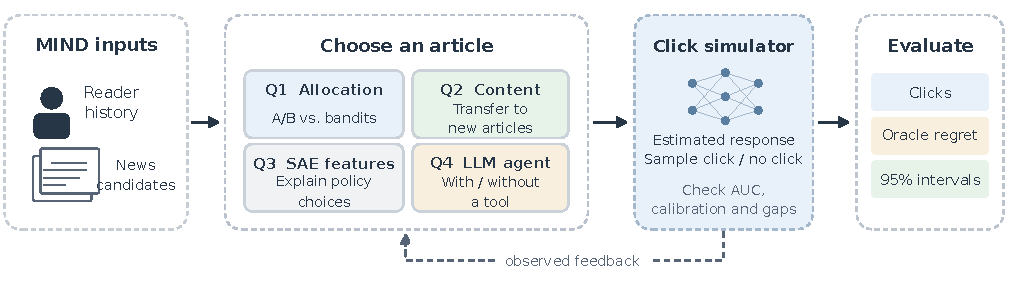
\includegraphics[width=\textwidth]{figures/project_overview.pdf}
\caption{Project overview. Policies choose an article, the shared click model samples feedback, and the policy updates from the observed click or non-click. Model-estimated probabilities define the simulator's oracle for measuring regret; policies do not observe those probabilities. Matched users and reward draws support paired comparisons across policies.}
\label{fig:concept}
\end{figure*}

\section{Related Work}
Bandits formalize the trade-off between exploration and exploitation \citep{lattimore2020bandit}, and Thompson sampling (TS) provides a strong Bayesian baseline \citep{chapelle2011empirical}. However, the comparison with A/B testing depends on test size and the traffic remaining after the test. \citet{feit2019test} show that profit-optimized test-and-roll can compete with adaptive allocation, motivating our comparison of train-tuned and power-based test lengths. We evaluate allocation reward rather than treatment-effect inference. For personalized news, \citet{li2010contextual} study contextual bandits with changing article pools. We use MIND's article text and logged clicks \citep{wu2020mind} to fit a response model with Qwen3 embeddings \citep{zhang2025qwen3}, while comparing separate policy representations including BGE-M3 \citep{chen2024m3}.

SAEs decompose activations into sparse features \citep{cunningham2024sparse}; pretrained Gemma Scope 2 models \citep{mcdougall2025scope} let us inspect a linear policy through feature importance and controlled removal. We interpret policy choices rather than language model circuits. For LLM decision-making, \citet{krishnamurthy2024explore} find that exploration depends strongly on prompting and summarized interaction histories. We extend that setting with an optional tool exposing posterior uncertainty and evaluate exploration failures and computational cost alongside regret.

\section{Validating the Shared Click Simulator}
\label{sec:simulator}
\subsection{Data and Temporal Separation}
We scaled from the proposed MIND-small setting to labeled MIND-large training and development logs, obtaining a catalog of 104,151 articles. The November 9--14, 2019 split contains 2,232,748 impressions and 83,507,374 displayed article--label pairs, while November 15 contains 376,471 impressions and 14,085,557 pairs. Their candidate-level CTRs are 4.052\% and 4.081\%, respectively. We fit candidate models on November 9--13, select their family and stopping epoch on November 14, refit on November 9--14, and evaluate on November 15. Although the repository calls November 15 \texttt{test}, we refer to it as the \emph{evaluation day}: it is MIND's labeled development split rather than the hidden-label benchmark test set. Users may overlap across periods.

\subsection{Click Model and Shared Interface}
Qwen3-Embedding-0.6B encodes article titles and abstracts, and normalized sums of history embeddings represent readers. Pair features combine content interactions and history affinities, without article IDs or popularity counts. We compare logistic, rank-64 bilinear, and neural models using training-fitted standardization and binary cross-entropy. The neural model has 256 ReLU hidden units. Validation selects the neural model at epoch two. Its validation AUC is 0.708, compared with 0.667 for logistic and 0.677 for bilinear prediction. The shared interface, \texttt{sim.prob\_matrix(users, articles)}, supplies user-by-article probabilities that environments cache before running policies. Cached probabilities decouple downstream experiments from model fitting; a synthetic backend remains planned.

\begin{figure*}[t]
\centering
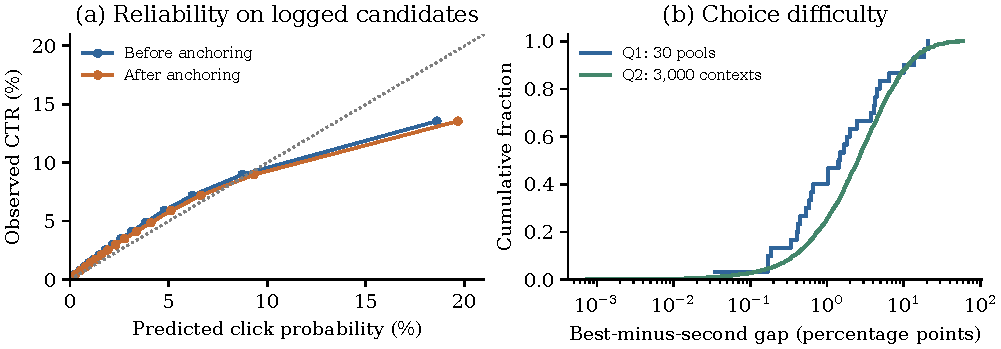
\includegraphics[width=\textwidth]{figures/simulator_validation.pdf}
\caption{Simulator checks beyond AUC. \textbf{(a)} Equal-count reliability bins show residual miscalibration after intercept anchoring; the dotted line is perfect calibration. \textbf{(b)} Best-minus-second-best probability gaps in the cached stationary Q1 setting ($K=10$) and 3,000 sampled Q2 contexts. These are gaps in learned simulator probabilities, not identified gaps in real user response.}
\label{fig:validation}
\end{figure*}

\begin{table}[!ht]
\caption{Evaluation-day click prediction. The constant predictor uses the earlier split's CTR. Anchoring changes probability values but preserves rankings. Lower log loss, Brier score, and ECE are better.}
\label{tab:simulator}
\centering
\small
\setlength{\tabcolsep}{3.2pt}
\begin{tabular}{lrrr}
\toprule
Metric & Constant & Neural & Anchored \\
\midrule
Global AUC & 0.500 & 0.733 & 0.733 \\
Impression AUC & --- & 0.686 & 0.686 \\
Log loss & 0.17051 & 0.15849 & 0.15837 \\
Brier score & 0.03915 & 0.03835 & 0.03843 \\
ECE (15 bins) & --- & 0.00958 & 0.00892 \\
Mean prediction (\%) & 4.052 & 3.797 & 4.052 \\
\bottomrule
\end{tabular}
\end{table}

\subsection{Validation and Decision Difficulty}
The selected model achieves global AUC 0.733 and impression-averaged AUC 0.686 (\cref{tab:simulator}), with the latter close to the range raised in the proposal feedback. For 757,273 evaluation pairs whose article IDs are absent from earlier candidate lists (5.38\% of candidates), AUC is 0.704; those IDs may nevertheless occur in earlier histories. The model underpredicts mean CTR, so the current simulator shifts its logits by $b=0.07291$ to match the earlier split's 4.052\% base rate over evaluation-day unlabeled pairs. This transductive adjustment uses evaluation covariates but no labels. ECE improves slightly while Brier score worsens slightly, and the highest-probability bin remains overconfident (\cref{fig:validation}). Matching the average rate therefore does not establish calibration for individual user--article pairs.

To characterize decision difficulty beyond AUC, we inspect the gaps between the best two articles, rather than only the spread of marginal probabilities. Across 30 ten-article Q1 pools, the median best-minus-second population gap is 1.45 percentage points (10th--90th percentiles: 0.19--10.37). Across 3,000 sampled Q2 user--pool contexts, the median gap is 2.53 points and 2.7\% fall below 0.1 point. Many simulated choices are well separated, potentially making learning easier than real recommendation. Section~\ref{sec:q1} tests sensitivity to this separation.

\section{Experimental Setup and Midway Results}
At each round, a policy chooses an article $a_t$ from the live set $\mathcal A_t$ and observes only its sampled click. Q1 measures population-average pseudo-regret,
\begin{equation}
R_T^{\mathrm{pop}}=\sum_{t=1}^{T}\left[\max_{a\in\mathcal A_t}\mu_t(a)-\mu_t(a_t)\right],
\end{equation}
while Q2 replaces $\mu_t(a)$ with $\hat p(u_t,a)$ for a per-user oracle. These regret scales are not directly comparable. CTR averages selected probabilities. We tune settings on earlier-day pools and evaluate on 30 later-day pools, sharing user arrivals and reward uniforms within each run. Reported intervals are 95\% Student-$t$ intervals across runs, with policy differences paired by run. They exclude uncertainty in the fitted simulator.

\subsection{Q1: Fixed Testing and Adaptive Allocation}
\label{sec:q1}
Fixed testing allocates traffic round-robin before committing to the largest empirical CTR, with its exploration fraction selected from $\{.01,.02,.05,.1,.2,.5\}$. A second baseline uses two-proportion power sizing with 5\% significance, 80\% power, and a train-selected relative effect of 20\% or 50\%. This pool-CTR sizing heuristic is not a validated multi-arm hypothesis test. Adaptive baselines include $\epsilon$-greedy, tuned UCB, Beta--Bernoulli TS, and discounted TS. We tune UCB's exploration multiplier, so its configuration differs from canonical UCB1.

\begin{figure*}[t]
\centering
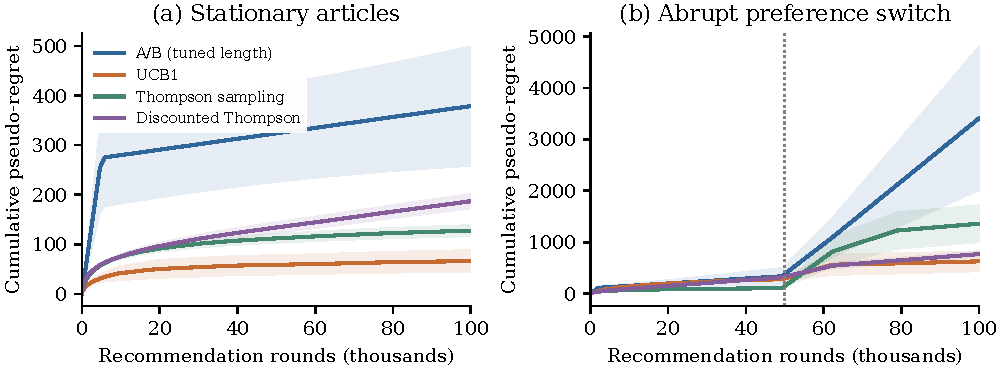
\includegraphics[width=\textwidth]{figures/q1_progress.pdf}
\caption{Q1 cumulative pseudo-regret for ten articles over 100,000 rounds. Shading shows 95\% intervals across 30 pools. Settings are tuned separately for each condition. The dotted line in panel (b) marks the abrupt switch at round 50,000. Curves share the population-average oracle within each panel.}
\label{fig:q1}
\end{figure*}

\begin{table}[t]
\caption{Q1 cumulative pseudo-regret over 30 evaluation pools. A/B length and UCB exploration are tuned on earlier-day pools separately for each condition. $K=10$ except the first row. Lower is better.}
\label{tab:q1}
\centering
\small
\setlength{\tabcolsep}{3.2pt}
\begin{tabular}{lrrr}
\toprule
Condition & A/B & UCB & TS \\
\midrule
$K=2$, $T=100$k & $\ci{39}{29}$ & $\ci{10}{4}$ & $\ci{19}{9}$ \\
$T=1$k & $\ci{29}{14}$ & $\ci{17}{4}$ & $\ci{28}{5}$ \\
$T=10$k & $\ci{179}{56}$ & $\ci{47}{16}$ & $\ci{80}{6}$ \\
$T=100$k & $\ci{379}{121}$ & $\ci{66}{23}$ & $\ci{128}{12}$ \\
Abrupt, $T=100$k & $\ci{3410}{1404}$ & $\ci{629}{202}$ & $\ci{1360}{367}$ \\
\bottomrule
\end{tabular}
\end{table}

For ten articles and 100,000 rounds, A/B testing incurs regret 379, compared with 128 for TS and 66 for UCB (\cref{tab:q1}); the paired A/B-minus-TS difference is $\ci{251}{124}$. At 1,000 rounds, however, the difference is only $\ci{0.8}{12.5}$. The power-based test loses $\ci{1203}{273}$ expected clicks at the longer horizon, showing the importance of test sizing. To stress-test adaptation, we also permute article response functions halfway through a run so that the best arm changes. This controlled abrupt switch penalizes fixed commitment (\cref{fig:q1}), while discounted TS achieves regret $\ci{770}{59}$ versus $\ci{1360}{367}$ for ordinary TS. These findings remain specific to the current environment.

To test sensitivity to nearly indistinguishable articles, we contract probabilities toward each user's mean,
\begin{equation}
P_\lambda(u,a)=\bar P_u+\lambda\bigl(P(u,a)-\bar P_u\bigr).
\end{equation}
This preserves user means and scales population gaps by $\lambda$. We use the same 30 pools and 10,000 rounds, frozen settings, and matched arrivals and reward uniforms. At one-quarter gaps, the A/B--TS difference becomes inconclusive (\cref{tab:gaps}), although UCB retains lower mean regret than TS at all three nonzero scales. We verify zero regret at $\lambda=0$ and reproduce the original cached runs at $\lambda=1$. Smaller gaps reduce both the cost of a wrong choice and the information available for learning, so declining absolute regret alone should not be interpreted as easier learning.

\begin{table}[t]
\caption{New gap-contraction experiment ($K=10$, $T=10$k). The final column is the paired A/B-minus-TS regret difference. At one-quarter gaps, its interval includes zero.}
\label{tab:gaps}
\centering
\small
\setlength{\tabcolsep}{4pt}
\begin{tabular}{rrrr}
\toprule
$\lambda$ & A/B regret & TS regret & A/B $-$ TS \\
\midrule
1.00 & $\ci{178.8}{55.9}$ & $\ci{79.5}{5.7}$ & $\ci{99.3}{55.9}$ \\
0.50 & $\ci{117.4}{30.4}$ & $\ci{78.2}{8.1}$ & $\ci{39.2}{27.5}$ \\
0.25 & $\ci{79.4}{22.0}$ & $\ci{72.2}{11.8}$ & $\ci{7.3}{16.2}$ \\
\bottomrule
\end{tabular}
\end{table}

\begin{table*}[t]
\caption{Q2 over 30 pools: 20 live articles, 20,000 rounds, and 2,000-round lifetimes. Features use $d=32$ (category: 18). Cold-start regret averages rounds whose oracle-best article is under 200 rounds old. CTR is expected; regret differences from per-article TS are paired.}
\label{tab:q2}
\centering
\small
\setlength{\tabcolsep}{5pt}
\begin{tabular}{llrrrr}
\toprule
Representation & Policy & Regret & Cold-start regret/round & CTR (\%) & Regret $-$ TS \\
\midrule
No content & Per-article TS & $\ci{1338}{28}$ & $\ci{.0562}{.0016}$ & 5.77 & --- \\
Category & LinUCB & $\ci{1490}{100}$ & $\ci{.0769}{.0051}$ & 5.01 & $\ci{152}{106}$ \\
BGE-M3 & LinUCB & $\ci{816}{58}$ & $\ci{.0429}{.0030}$ & 8.38 & $\ci{-522}{68}$ \\
Gemma-3-1B dense, L23 & LinUCB & $\ci{753}{36}$ & $\ci{.0408}{.0020}$ & 8.69 & $\ci{-585}{39}$ \\
Gemma-3-1B SAE, L17 & LinUCB & $\ci{920}{55}$ & $\ci{.0515}{.0029}$ & 7.86 & $\ci{-418}{47}$ \\
\bottomrule
\end{tabular}
\end{table*}

\subsection{Q2: Content under Article Turnover}
We keep 20 articles live over 20,000 rounds, replace one every 100 rounds (2,000-round lifetimes), and sample 2,000 users per run. Shared LinUCB and linear TS use $\phi(u,a)=[1;x_a;h_u\odot x_a]$, where $h_u$ averages history features, while per-article TS starts each arrival with a Beta$(1,1)$ prior. Representations comprise categories, BGE-M3, mean-pooled Gemma-3-1B/12B activations, and token-averaged Gemma Scope 2 codes. Dense PCA and SAE coordinate selection use earlier articles. Scalar normalization uses the unlabeled catalog; layer and exploration selection use earlier-day simulations. We report 32 features, except the 18-dimensional category representation. The simulator-sharing Qwen3 comparison is retained as a diagnostic in the saved results.

Gemma-3-1B dense features reduce regret relative to per-article TS by $\ci{585}{39}$, approximately 44\% of its mean (\cref{tab:q2}), whereas categories provide no similar benefit. SAE configurations improve over TS but incur approximately 168 additional regret relative to the dense configurations, with paired intervals $\ci{168}{55}$ for 1B and $\ci{168}{67}$ for 12B. Because selected layers and policies differ, this is a configuration-level comparison rather than an isolated effect of sparsity. At 500-round lifetimes, TS regret increases to $\ci{1716}{32}$ versus $\ci{894}{33}$ for Gemma-3-1B dense features, supporting further investigation of content transfer under turnover. However, ``new'' currently means unseen by the online policy: arriving articles may have appeared in simulator fitting or feature preprocessing. A strict article-ID holdout remains necessary before claiming generalization to previously unseen articles.

\subsection{Q3--Q4: Initial Feasibility Results}
Our interpretability analysis implements train-ranked importance and retraining ablations. For exploratory Gemma-3-12B SAE layer 41, eight of the ten highest-ranked features have Neuronpedia descriptions, and removing the top eight before retraining costs $\ci{111}{51}$ more regret than random eight-feature removal. At four features, that difference is only $\ci{6}{29}$. Feature relevance does not yet establish semantic faithfulness: the human label-check sheets remain unannotated, and post-hoc checks currently rescore linear predictions rather than the full UCB bonus. Both label correctness and the complete decision rule require validation.

Initial Gemma-3-12B-IT experiments use summarized click counts, 500 rounds, and 30 pools. For ten articles, regret is $\ci{15.2}{4.2}$ without the statistics tool, $\ci{9.3}{2.6}$ with it, and $\ci{14.7}{2.6}$ for TS; the paired tool-minus-TS difference is $\ci{-5.4}{2.8}$. The tool exposes posterior means, credible bounds, and probabilities of being best. Runs allocating at least 90\% of the final 250 rounds to one suboptimal article fall from 70\% to 3\%, while tokens per 1,000 decisions rise from 551,000 to 932,000. This suggests that explicit uncertainty helps this agent explore, but a direct statistics-based tool policy remains necessary to determine what the LLM contributes beyond the tool itself.

\balance
\section{Current Limitations}
The model learns from production exposures, which do not identify outcomes for arbitrary recommendations. For 2,125 articles with at least 100 exposures, simulated and logged CTR correlate at $\rho=0.56$ (Spearman), but reader selection confounds this diagnostic. Calibration choices and exploratory analyses also used the evaluation day during development, so it is not an untouched confirmation set. The environment assumes immediate feedback, fixed histories, single-article displays, and synthetic turnover, excluding slate effects and long-term response. Intervals condition on one simulator, so these are preliminary comparisons rather than real-world CTR improvements. We will test which conclusions survive alternative modeling choices.

\section*{Work Before the Final Submission}
By November 15, we will add a synthetic backend with controlled CTRs and gaps, refit on earlier temporal partitions, calibrate on a disjoint block, and reserve a confirmation partition. The existing last-day alternative used a model already refitted on that day; the revised protocol will separate these stages and record provenance. We will extend simulator sensitivity checks to Q2. By November 22, we will add strict article-ID holdouts, reward-aware test sizing, and batched allocation, then compare dense and SAE features at matched layers with random-feature controls and paired uncertainty estimates.

By November 29, we will complete human feature-label checks and full-UCB interventions, compare LLM decisions with posterior-based tool policies, vary headline order and prompts, and report runtime and token use. Additional models depend on compute availability. We will consolidate validated findings into the final report by December 7 and build the interactive demonstration for the December 9 poster session, showing recommendations, regret, and explanatory features or statistics. Off-policy evaluation remains a stretch goal requiring known logging propensities.

\bibliography{paper}
\bibliographystyle{icml2026}
\end{document}
